\documentclass[en]{../../../eplsummary}

\usepackage{multicol}
\usepackage{pgfplots}

\hypertitle{Nonlinear programming}{8}{INMA}{2460}
{Benoît Legat}
{Yurii Nesterov}

\begin{center}
  ``The main fact, which should be known to any person dealing with optimization models,
  is that, in general, \emph{the optimization problems are unsolvable}.''
  \hfill\cite[p.~5]{nesterov1998introductory}
\end{center}

\section{The World of Nonlinear Optimization}
We are interested in the problem
\begin{align*}
  \min & f_0(x)\\
  f_j(x) & \leq 0 & j = 1, \ldots, m\\
  x & \in S.
\end{align*}
where $f_0$ is the \emph{objective} function,
the vector function $f(x) = (f_1(x), \ldots,f_m(x))$ is called the \emph{functional constraint},
the set $S$ is called the \emph{basic feasible set} and the set
\[ Q = \{\, x \in S \mid f_j(x) \leq 0, j = 1, \ldots, m \, \} \]
is called the \emph{feasible set} of the optimization problem.

$S$ stands for \emph{structural} constraints, like non-negativity or boundedness of some variables.
% TODO link that to chapter 4

\begin{itemize}
  \item It is called \emph{unconstrained} if $Q \equiv S \equiv \Rn$ and \emph{constrained} otherwise.
  \item It is called \emph{smooth} if all the $f_i$ are differentiable and \emph{nonsmooth} otherwise.
\end{itemize}

A \emph{method} $\mathcal{M}$ for a \emph{class} $\mathcal{F}$ is given as input a problem $\mathcal{P}$ of $\mathcal{F}$.
Since $\mathcal{M}$ deals with the whole class $\mathcal{F}$,
it does not have the complete description of the problem $\mathcal{P}$ but rather the description of the class $\mathcal{F}$.
In addition it has access to an oracle $\mathcal{O}$ to collect specific information about $\mathcal{P}$.

The pair $(\mathcal{F}, \mathcal{O})$ defines a \emph{model}.
The \emph{peformance} of a method $\mathcal{M}$ on a model $(\mathcal{F}, \mathcal{O})$ is its performance on the \emph{worst} problem $\mathcal{P}_w$ of $\mathcal{F}$ for $\mathcal{M}$.

Once we define what ``a solution $x$ with accuracy $\epsilon$'' means (e.g. $\|x - x^*\| \leq \epsilon$, $|f(x)-f(x^*)| \leq \epsilon$, ...) % TODO do a list
we can define the complexity of the problem $\mathcal{P}$ for the method $\mathcal{M}$
\begin{description}
  \item[Analytical complexity]
    The number of calls to the oracle required for an accuracy $\epsilon$.
  \item[Arithmetical complexity]
    The number of arithmetic operations required for an accuracy $\epsilon$,
    including operations done by the oracle and by the method.
\end{description}

We will analyse three type of oracle of input $x \in \mathbb{R}^n$%TODO on les analyse vraiment tous ?
\begin{description}
  \item[Zero-order oracle] outputs the value $f(x)$.
  \item[First-order oracle] outputs the value $f(x)$ and the gradient $f'(x)$.
  \item[Second-order oracle] outputs the value $f(x)$, the gradient $f'(x)$ and the Hessian $f''(x)$.
\end{description}

\subsection{Global optimization}
The purpose of this section is to show that global optimization is impossible and we should work on smaller classes of problems.

Clearly, if we do not make any continuity assumption on the objective, the oracle won't give us a lot of information.
Also, since we do not consider that $f$ is convex, we cannot search for the \emph{global} optimal solution in an infinite domain.

Let % TODO the objective is f or f_0 ? f is (f_1, ..., f_m)...
\[ Q = B_n = \{\, x \in \Rn \mid 0 \leq x_i \leq 1, i = 1, \ldots, n \,\} \]
and $f_0$ be $L$-Lipschitz continuous
\begin{align*}
  |f(x) - f(y)| & \leq L\|x - y\| & \forall x,y \in B_n.
\end{align*}
We consider here a Zero-order oracle but the lower complexity bound will be the same for a smooth $f_0$ of for higher order oracle~\cite[p.~18]{nesterov1998introductory}.

The grid method $\mathcal{G}(p)$ consists in calling the oracle at all the $(p+1)^n$ points
of the set $\{0,1/p,2/p,\ldots,1\}^n$ and return the point of the grid giving the minimum value for the objective $f_0$.

\begin{tabular}{lll} % TODO find exact bounds
  $L$-Lipschitz with norm & $\mathcal{G}$ & Lower\\
  2
  & $\big(\lfloor \frac{L\sqrt{n}}{2\epsilon} \rfloor + 2\big)^n$
  & $\big(\lfloor \frac{L}{2\epsilon} \rfloor\big)^n$\\
  $\infty$
  & $\big(\lfloor \frac{L}{2\epsilon} \rfloor + 2\big)^n$
  & $\big(\lfloor \frac{L}{2\epsilon} \rfloor\big)^n$
\end{tabular}

\subsection{Nonlinear optimization}
\subsubsection{Function classes}
If $f$ is differentiable at $\bar{x}$ then for $y \in \Rn$ we have
\[ f(x) = f(\bar{x}) + \langle f'(\bar{x}), y-\bar{x}\rangle + o(\|y-\bar{x}\|) \]
where $o(r)$ is some function of $r > 0$ such that $\lim_{r \downarrow 0} \frac{1}{r}o(r) = 0$ and $o(0) = 0$.

\begin{mynota}
  We denote by $C^{k,p}_L(Q)$ the class of functions $f$ that are $k$ times continuously differentiable on $Q$
  and its $p$th derivative is Lipschitz continuous on $Q$ with the constant $L$:
  \[ \| f^{(p)}(x) - f^{(p)}(y) \| \leq L \| x - y \| \]
  for all $x,y \in Q$.
\end{mynota}

We have seen that we cannot win the game of optimization in General or with a Lipschitz continuous fonction.
Any function can be approximated as close as possible with a smooth function so with need First or Second order Lipschitz.
\paragraph{First order Lipschitz}
\begin{mylem}
  A function $f \in C^2$ belongs to $C^{2,1}_L(\Rn) \subseteq C^{1,1}_L(\Rn)$ if and only if
  \[ \| f''(x) \| \leq L \]
  for all $x \in \Rn$.
\end{mylem}

\begin{multicols}{2}
  \begin{myprop}
    Let $f \in C^{1,1}_L$. Then for any $x,y \in \Rn$ we have
    \[ | f(y) - f(x) - \langle f'(x), y-x \rangle| \leq \frac{L}{2} \|y - x\|^2. \] % TODO image
  \end{myprop}

  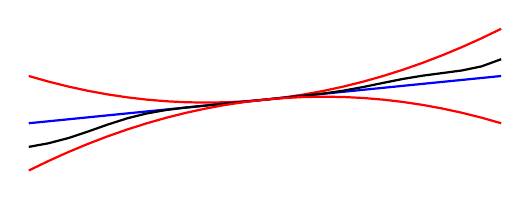
\begin{tikzpicture}[x=3cm,y=0.6cm]
    \draw[color=red, thick, domain=-1:1] plot
    (\x, {\x/2+(\x)^2});
    \draw[color=blue, thick, domain=-1:1] plot
    (\x, {\x/2});
    \draw[thick, domain=-1:1] plot
    (\x, {(\x)^3/2 - \x*\x*sin(60+\x*420)/6+\x/2});
    \draw[color=red, thick, domain=-1:1] plot
    (\x, {\x/2-(\x)^2});
  \end{tikzpicture}
\end{multicols}

\paragraph{Second order Lipschitz}
We have the exact same property thant for First order Lipschitz with $f'$ since $f'$ is first order Lipschitz
\begin{myprop}
  Let $f \in C^{2,2}_M$. Then for any $x,y \in \Rn$ we have
  \[ | f'(y) - f'(x) - \langle f''(x), y-x \rangle| \leq \frac{M}{2} \|y - x\|^2. \]
\end{myprop}
\begin{mycorr}
  Let $f \in C^{2,2}_M$. Then for any $x,y \in \Rn$ we have
  \[ f''(x) - M\|y-x\|I_n \leq f''(y) \leq f''(x) - M\|y-x\|I_n. \]
\end{mycorr}

\subsection{Local methods in unconstrained minimization}
\begin{mydef}
  We call a sequence $\{a_k\}_{k=1}^\infty$ a \emph{relaxation sequence} if $a_{k+1} \leq a_k$ for all $k \geq 0$.
\end{mydef}
Remember that every non-increasing sequence bounded from below is Cauchy.
If we generate a relaxation sequence $\{f(x_k)\}_{k=0}^\infty$ and $f$ is bounded from below it converges.

\subsubsection{Gradient method}
The Gradient method iteration is
\[ x_{k+1} = x_k - h_kf'(x_k). \]
If follows the steepest descent $f'(x_k)$ which is a decrease so $\{f(x_k)\}_{k=0}^\infty$ is a relaxation sequence.
$h_k$ can be fixed a priori to constant or a function of $k$, e.g. $h/\sqrt{k+1}$ for some constant $h$.
But it can also be computed at each iteration.
Theoritically, we would like to pick
\[ h_k = \argmin_{h \geq 0} f(x_k - hf'(x_k)). \]
In practice we rather use the Goldstein-Armijo rule
\[ \alpha\langle f'(x_k), x_k - x_{k+1}\rangle \leq f(x_k) - f(x_{k+1}) \leq \beta\langle f'(x_k), x_k - x_{k+1}\rangle \]
\begin{multicols}{2}
  \noindent
  which in the case of the Gradient method is
  \[ \alpha h_k\|f'(x_k)\|^2 \leq f(x_k) - f(x_{k+1}) \leq \beta h_k\|f'(x_k)\|^2 \]
  since $x_k - x_{k+1} = -h_kf'(x_k)$.

  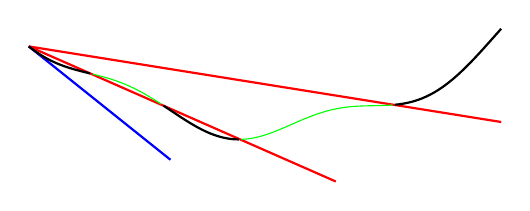
\begin{tikzpicture}[x=3cm,y=0.6cm]
    \draw[color=red, thick, domain=0:2] plot
    (\x, {-0.2*4*\x+1.75});
    \draw[color=red, thick, domain=0:1.3] plot
    (\x, {-0.55*4*\x+1.75});
    \draw[color=blue, thick, domain=0:0.6] plot
    (\x, {-4*\x+1.75});
    \draw[thick, domain=0:0.26] plot
    (\x, {2*(\x-1)^2 - cos(\x*420)/4});
    \draw[green, domain=0.27:0.56] plot
    (\x, {2*(\x-1)^2 - cos(\x*420)/4});
    \draw[thick, domain=0.57:0.89] plot
    (\x, {2*(\x-1)^2 - cos(\x*420)/4});
    \draw[green, domain=0.90:1.54] plot
    (\x, {2*(\x-1)^2 - cos(\x*420)/4});
    \draw[thick, domain=1.55:2] plot
    (\x, {2*(\x-1)^2 - cos(\x*420)/4});
  \end{tikzpicture}
\end{multicols}

\section{Smooth Convex Programming}
\section{Nonsmooth Convex Programming}
\section{Structural Programming}
%In Structural programming, we do not consider constraints as black blox.
%We use the specificity in their structure to remplace them by barriers in the objective.
%The remaining objective is solved using the Newton['s]? scheme.

\biblio
\end{document}
